\documentclass{standalone}
\usepackage{tikz}
\usetikzlibrary{patterns, positioning}


\begin{document}
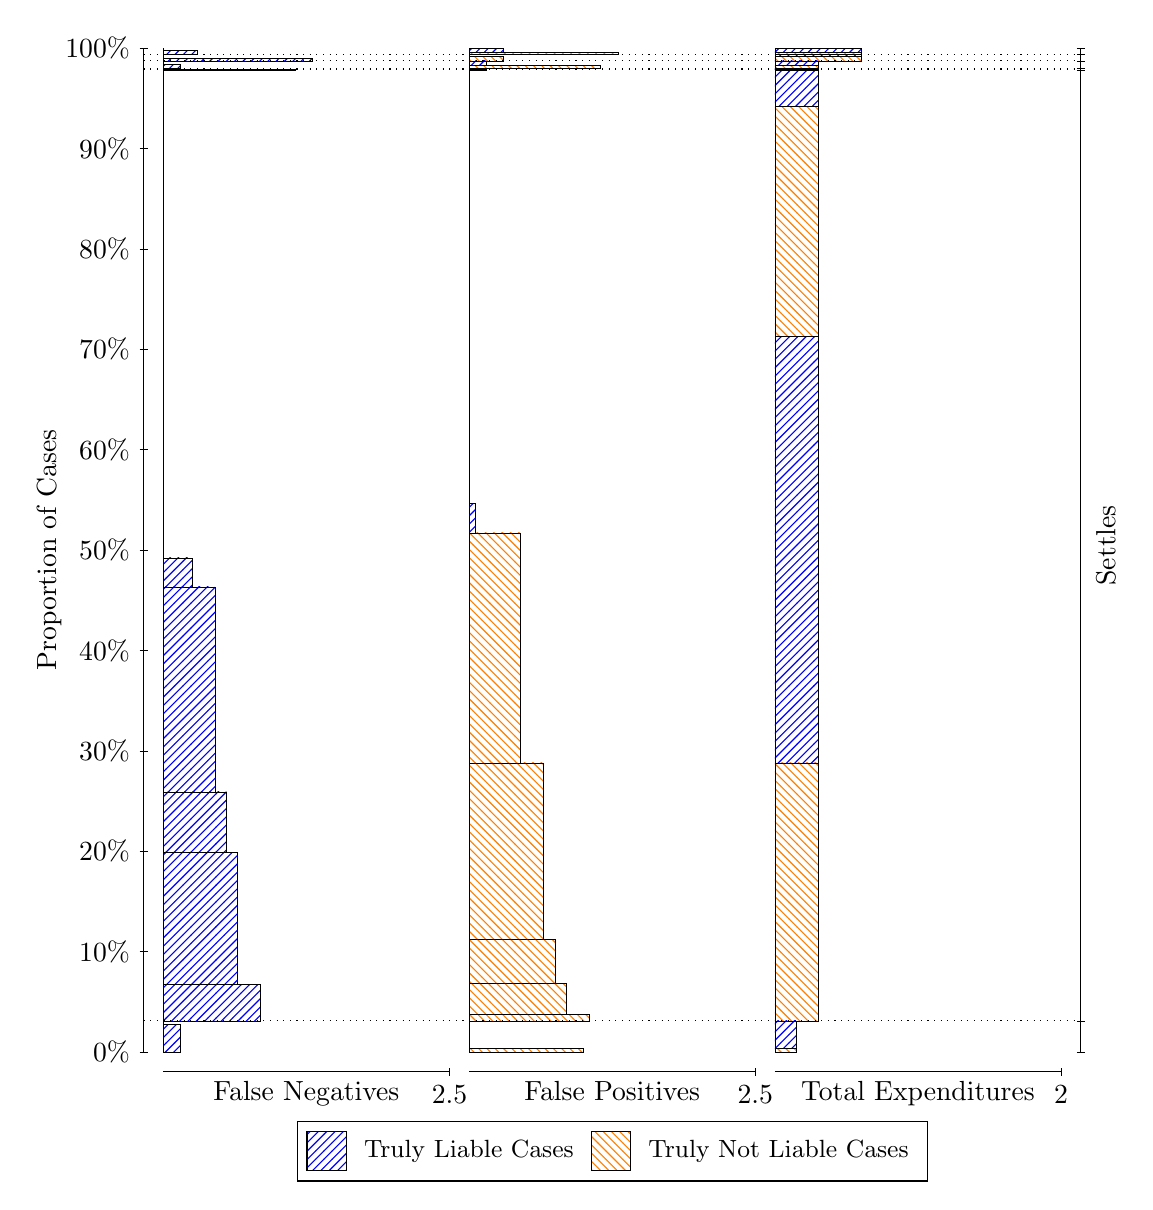
\begin{tikzpicture}
\draw[black, very thin] (1.5,1.75) -- (1.5,14.5);
\node[rotate=90, text=black, anchor=center] at (0.3, 8.125) {Proportion of Cases};
\draw[black, very thin] (1.45,1.75) -- (1.55,1.75);
\node[text=black, anchor=east] at (1.45, 1.75) {0\%};
\draw[black, very thin] (1.45,3.025) -- (1.55,3.025);
\node[text=black, anchor=east] at (1.45, 3.025) {10\%};
\draw[black, very thin] (1.45,4.3) -- (1.55,4.3);
\node[text=black, anchor=east] at (1.45, 4.3) {20\%};
\draw[black, very thin] (1.45,5.575) -- (1.55,5.575);
\node[text=black, anchor=east] at (1.45, 5.575) {30\%};
\draw[black, very thin] (1.45,6.85) -- (1.55,6.85);
\node[text=black, anchor=east] at (1.45, 6.85) {40\%};
\draw[black, very thin] (1.45,8.125) -- (1.55,8.125);
\node[text=black, anchor=east] at (1.45, 8.125) {50\%};
\draw[black, very thin] (1.45,9.4) -- (1.55,9.4);
\node[text=black, anchor=east] at (1.45, 9.4) {60\%};
\draw[black, very thin] (1.45,10.675) -- (1.55,10.675);
\node[text=black, anchor=east] at (1.45, 10.675) {70\%};
\draw[black, very thin] (1.45,11.95) -- (1.55,11.95);
\node[text=black, anchor=east] at (1.45, 11.95) {80\%};
\draw[black, very thin] (1.45,13.225) -- (1.55,13.225);
\node[text=black, anchor=east] at (1.45, 13.225) {90\%};
\draw[black, very thin] (1.45,14.5) -- (1.55,14.5);
\node[text=black, anchor=east] at (1.45, 14.5) {100\%};

\draw[black, very thin] (13.4,1.75) -- (13.4,14.5);
\draw[black, very thin] (13.35,1.75) -- (13.45,1.75);
\node[anchor=west] at (13.35, 1.75) {};
\draw[black, very thin] (13.35,2.1454) -- (13.45,2.1454);
\node[anchor=west] at (13.35, 2.1454) {};
\draw[black, very thin] (13.35,14.223) -- (13.45,14.223);
\node[anchor=west] at (13.35, 14.223) {};
\draw[black, very thin] (13.35,14.241) -- (13.45,14.241);
\node[anchor=west] at (13.35, 14.241) {};
\draw[black, very thin] (13.35,14.336) -- (13.45,14.336);
\node[anchor=west] at (13.35, 14.336) {};
\draw[black, very thin] (13.35,14.421) -- (13.45,14.421);
\node[anchor=west] at (13.35, 14.421) {};
\draw[black, very thin] (13.35,14.5) -- (13.45,14.5);
\node[anchor=west] at (13.35, 14.5) {};

\draw[black, very thin, pattern color=blue, pattern=north east lines] (1.75,1.75) rectangle (1.968,2.1038);
\draw[black, very thin, pattern color=orange, pattern=north west lines] (1.75,2.1038) rectangle (1.75,2.1454);
\draw[black, very thin, pattern color=blue, pattern=north east lines] (1.75,2.1454) rectangle (2.9853,2.6091);
\draw[black, very thin, pattern color=blue, pattern=north east lines] (1.75,2.6091) rectangle (2.6947,4.2839);
\draw[black, very thin, pattern color=blue, pattern=north east lines] (1.75,4.2839) rectangle (2.5493,5.0533);
\draw[black, very thin, pattern color=blue, pattern=north east lines] (1.75,5.0533) rectangle (2.404,7.6566);
\draw[black, very thin, pattern color=blue, pattern=north east lines] (1.75,7.6566) rectangle (2.1133,8.0253);
\draw[black, very thin, pattern color=orange, pattern=north west lines] (1.75,8.0253) rectangle (1.75,14.223);
\draw[black, very thin, pattern color=blue, pattern=north east lines] (1.75,14.223) rectangle (3.4213,14.231);
\draw[black, very thin, pattern color=orange, pattern=north west lines] (1.75,14.231) rectangle (1.75,14.241);
\draw[black, very thin, pattern color=blue, pattern=north east lines] (1.75,14.241) rectangle (1.968,14.295);
\draw[black, very thin, pattern color=orange, pattern=north west lines] (1.75,14.295) rectangle (1.75,14.336);
\draw[black, very thin, pattern color=blue, pattern=north east lines] (1.75,14.336) rectangle (3.6393,14.364);
\draw[black, very thin, pattern color=orange, pattern=north west lines] (1.75,14.364) rectangle (1.75,14.421);
\draw[black, very thin, pattern color=blue, pattern=north east lines] (1.75,14.421) rectangle (2.186,14.472);
\draw[black, very thin, pattern color=orange, pattern=north west lines] (1.75,14.472) rectangle (1.75,14.5);
\draw[black, very thin, pattern color=orange, pattern=north west lines] (5.6333,1.75) rectangle (7.0867,1.7916);
\draw[black, very thin, pattern color=blue, pattern=north east lines] (5.6333,1.7916) rectangle (5.6333,2.1454);
\draw[black, very thin, pattern color=orange, pattern=north west lines] (5.6333,2.1454) rectangle (7.1593,2.2263);
\draw[black, very thin, pattern color=orange, pattern=north west lines] (5.6333,2.2263) rectangle (6.8687,2.6194);
\draw[black, very thin, pattern color=orange, pattern=north west lines] (5.6333,2.6194) rectangle (6.7233,3.1847);
\draw[black, very thin, pattern color=orange, pattern=north west lines] (5.6333,3.1847) rectangle (6.578,5.4207);
\draw[black, very thin, pattern color=orange, pattern=north west lines] (5.6333,5.4207) rectangle (6.2873,8.3435);
\draw[black, very thin, pattern color=blue, pattern=north east lines] (5.6333,8.3435) rectangle (5.706,8.7122);
\draw[black, very thin, pattern color=blue, pattern=north east lines] (5.6333,8.7122) rectangle (5.6333,14.223);
\draw[black, very thin, pattern color=orange, pattern=north west lines] (5.6333,14.223) rectangle (5.8513,14.233);
\draw[black, very thin, pattern color=blue, pattern=north east lines] (5.6333,14.233) rectangle (5.6333,14.241);
\draw[black, very thin, pattern color=orange, pattern=north west lines] (5.6333,14.241) rectangle (7.3047,14.281);
\draw[black, very thin, pattern color=blue, pattern=north east lines] (5.6333,14.281) rectangle (5.8513,14.336);
\draw[black, very thin, pattern color=orange, pattern=north west lines] (5.6333,14.336) rectangle (6.0693,14.392);
\draw[black, very thin, pattern color=blue, pattern=north east lines] (5.6333,14.392) rectangle (5.6333,14.421);
\draw[black, very thin, pattern color=orange, pattern=north west lines] (5.6333,14.421) rectangle (7.5227,14.449);
\draw[black, very thin, pattern color=blue, pattern=north east lines] (5.6333,14.449) rectangle (6.0693,14.5);
\draw[black, very thin, pattern color=orange, pattern=north west lines] (9.5167,1.75) rectangle (9.7892,1.7916);
\draw[black, very thin, pattern color=blue, pattern=north east lines] (9.5167,1.7916) rectangle (9.7892,2.1454);
\draw[black, very thin, pattern color=orange, pattern=north west lines] (9.5167,2.1454) rectangle (10.062,5.4207);
\draw[black, very thin, pattern color=blue, pattern=north east lines] (9.5167,5.4207) rectangle (10.062,10.837);
\draw[black, very thin, pattern color=orange, pattern=north west lines] (9.5167,10.837) rectangle (10.062,13.76);
\draw[black, very thin, pattern color=blue, pattern=north east lines] (9.5167,13.76) rectangle (10.062,14.223);
\draw[black, very thin, pattern color=orange, pattern=north west lines] (9.5167,14.223) rectangle (10.062,14.233);
\draw[black, very thin, pattern color=blue, pattern=north east lines] (9.5167,14.233) rectangle (10.062,14.241);
\draw[black, very thin, pattern color=orange, pattern=north west lines] (9.5167,14.241) rectangle (10.062,14.281);
\draw[black, very thin, pattern color=blue, pattern=north east lines] (9.5167,14.281) rectangle (10.062,14.336);
\draw[black, very thin, pattern color=orange, pattern=north west lines] (9.5167,14.336) rectangle (10.607,14.392);
\draw[black, very thin, pattern color=blue, pattern=north east lines] (9.5167,14.392) rectangle (10.607,14.421);
\draw[black, very thin, pattern color=orange, pattern=north west lines] (9.5167,14.421) rectangle (10.607,14.449);
\draw[black, very thin, pattern color=blue, pattern=north east lines] (9.5167,14.449) rectangle (10.607,14.5);
\draw[black, dotted] (1.5,2.1454) -- (13.4,2.1454);
\draw[black, dotted] (1.5,14.223) -- (13.4,14.223);
\draw[black, dotted] (1.5,14.241) -- (13.4,14.241);
\draw[black, dotted] (1.5,14.336) -- (13.4,14.336);
\draw[black, dotted] (1.5,14.421) -- (13.4,14.421);
\draw[black, very thin] (1.75,1.5) -- (5.3833,1.5);
\node[text=black, anchor=north] at (3.5667, 1.5) {False Negatives};
\draw[black, very thin] (5.3833,1.45) -- (5.3833,1.55);
\node[text=black, anchor=north] at (5.3833, 1.45) {2.5};

\draw[black, very thin] (5.6333,1.5) -- (9.2667,1.5);
\node[text=black, anchor=north] at (7.45, 1.5) {False Positives};
\draw[black, very thin] (9.2667,1.45) -- (9.2667,1.55);
\node[text=black, anchor=north] at (9.2667, 1.45) {2.5};

\draw[black, very thin] (9.5167,1.5) -- (13.15,1.5);
\node[text=black, anchor=north] at (11.333, 1.5) {Total Expenditures};
\draw[black, very thin] (13.15,1.45) -- (13.15,1.55);
\node[text=black, anchor=north] at (13.15, 1.45) {2};


\node[text=black, centered, rotate=90] at (13.72, 8.1844) {Settles};





\draw (7.449999999999999,1.5) node[draw=none] (baseCoordinate) {};
\begin{scope}[align=center]
        \matrix[scale=0.5, draw=black, below=0.5cm of baseCoordinate, nodes={draw}, column sep=0.1cm]{
            \node[rectangle, draw, minimum width=0.5cm, minimum height=0.5cm, pattern color=blue, pattern=north east lines] {}; &
            \node[draw=none, font=\small, text=black] (B) {Truly Liable Cases}; &
            \node[rectangle, draw, minimum width=0.5cm, minimum height=0.5cm, pattern color=orange, pattern=north west lines] {}; &
            \node[draw=none, font=\small, text=black] (B) {Truly Not Liable Cases}; \\
            };
\end{scope}

\end{tikzpicture}
\end{document}